\documentclass[12pt]{article}
\usepackage{graphicx}
\usepackage{amssymb} %math
\usepackage{amsmath} %math alignment
\usepackage{lineno}
\usepackage{lscape}
\usepackage{authblk}
\usepackage{xcolor}
\usepackage{soul}
\usepackage{caption}
\usepackage{hyperref} %hyper link

\usepackage{geometry}
\geometry{left=1.0in,right=1.0in,top=1.0in,bottom=1.0in} % set up margin
\usepackage{setspace}   %Allows double spacing with the \doublespacing command
\usepackage{booktabs}  % table
\usepackage{siunitx} 
\usepackage{multirow} % table
\usepackage{float}
\usepackage{pdflscape}
\usepackage{adjustbox} % resize figures and tables
\usepackage{import} %% for \subimport <- table 

\usepackage{rotating} %% for rotate orientation
\usepackage{bm}

\usepackage{tikz} 
\def\checkmark{\tikz\fill[scale=0.4](0,.35) -- (.25,0) -- (1,.7) -- (.25,.15) -- cycle;}  % Checkmark

\usepackage{natbib} %bib package
\bibliographystyle{apsr}

\usepackage{ntheorem}  % Hypothsis
\makeatletter %
\newtheoremstyle{hypotheses}%
  {\item[\hskip\labelsep \theorem@headerfont ##1##2\theorem@separator]}%
  {\item[\hskip\labelsep \theorem@headerfont ##1##2\ (##3)\theorem@separator]}
\makeatother

\theoremstyle{hypotheses}
\newtheorem{hyp}{H} 
\newtheorem{subhyp}{H}
   \renewcommand\thesubhyp{\thehyp\alph{subhyp}}

\begin{document}


\title{How to Use Overleaf \thanks{Thank you thank you thank you. All views expressed in this paper are....}}
%%%%%%%%%%%%%%%%%%%%%%
%%%%% First Page %%%%%
%%%%%%%%%%%%%%%%%%%%%%

\author{Ichiro Suzuki\thanks{Seattle Mariners}}
\author{Rui Hachimura\thanks{Washington Wizards}}
\affil{University of Washington}
\date{}
\maketitle

\begin{abstract}
Overleaf is a collaborative cloud-based \LaTeX editor used for writing, editing and publishing scientific documents. It partners with[clarification needed] a wide range of scientific publishers to provide official journal \LaTeX templates, and direct submission links. Overleaf was originally launched in 2012 as WriteLaTeX by the company WriteLaTeX Limited, co-founded by John Hammersley and John Lees-Miller. Both are mathematicians and were inspired by their own experiences in academia to create a better solution for collaborative scientific writing. They started developing WriteLaTeX from 2011. They launched the beta version of Overleaf on the January 16, 2014, at their first #FuturePub event held at the British Library in London.
\vspace{0in}\\
%\noindent\textbf{Keywords:} key1, key2, key3\\
%\vspace{0in}\\
%\noindent\textbf{JEL Codes:} key1, key2, key3\\
\bigskip
\end{abstract}
% If you want to make the first page as page number zero 
% \setcounter{page}{0} 

\clearpage


\doublespacing
% \linespread{1.5} 
% Another way to do double space 

%%%%%%%%%%%%%%%%%%%%
%%%%% Body %%%%%
%%%%%%%%%%%%%%%%%%%%

\section{Introduction}
GitHub, Inc. is a subsidiary of Microsoft which provides hosting for software development and version control using Git. It offers the distributed version control and source code management (SCM) functionality of Git, plus its own features. It provides access control and several collaboration features such as bug tracking, feature requests, task management, continuous integration and wikis for every project. Headquartered in California, it has been a subsidiary of Microsoft since 2018\footnote{ Excerpt from \href{https://en.wikipedia.org/wiki/GitHub}{wikipedia}}.  To begin Git and GitHub, go this \href{https://happygitwithr.com/}{LINK}.


\section*{Introduction}
With asterisk, the section title will not be numbered (I prefer this).


\section*{Literature Review\footnote{ \url{https://en.wikipedia.org/wiki/Ichiro_Suzuki}}}
Due to an agreement between Japanese baseball and the MLB, Ichiro was not allowed to play in the United States before 2001. His move to the United States was viewed with some interest because he was among the first Japanese position players to play for an MLB team. In the same way that many Japanese teams had considered the 18-year-old Ichiro too small to draft in 1992, many Americans believed he would prove too frail to succeed against Major League pitching or endure the longer 162-game season. Ichiro made an auspicious debut with Seattle, and in the Mariners' eighth game revealed his tremendous throwing arm by gunning down Oakland's Terrence Long, who had tried to advance from first to third on a teammate's single to right field. That play would be dubbed "The Throw" by Japanese media covering Ichiro's progress \citep{KinBa14, Svolik2020WhenIncumbents}.

After expressing no preference as to a uniform number, Ichiro was issued #51 by the Mariners. He was initially hesitant because it had previously been worn by pitching star Randy Johnson. To avoid insulting Johnson, Ichiro sent a personal message to the pitcher promising not to "bring shame" to the uniform. His trepidation was unfounded, as he had a remarkable 2001 season, accumulating a rookie-record 242 hits, the most by any MLB player since 1930. His perennial Gold Glove fielding led Safeco's right field to be dubbed "Area 51".


\section*{Theory}
With a .350 batting average and 56 stolen bases, Ichiro was the first player to lead his league in both categories since Jackie Robinson in 1949. The season included hitting streaks of 25 and 23 games, an appearance on the cover of Sports Illustrated, and intense media attention on both sides of the Pacific. Fans from Japan were taking \$2,000 baseball tours, sometimes flying in and out of the U.S. just to watch Ichiro's games. More than 150 Japanese reporters and photographers were given media access. Safeco Field's sushi stands began selling "Ichirolls", a spicy tuna roll served with wasabi and ginger.

\bigskip
\begin{hyp}
Eating: As the number of democracies increases, the effect of the level of GDP per capita on appetite diminishes.  
\end{hyp}

Aided by Major League Baseball's decision to allow All-Star voting in Japan, Ichiro was the first rookie to lead all players in voting for the All-Star Game. That winter, he won the American League Most Valuable Player and the Rookie of the Year awards, becoming only the second player in MLB history (after Fred Lynn) to receive both honors in the same season. Ichiro is also the only player in major league history to have won an MVP, Rookie of the Year, Gold Glove Award, Silver Slugger Award, all while starting in the All-Star Game in the same season.

\bigskip
\begin{hyp}
Learning: Elite and middle class learn from the neighbor democratic countries: As the number of democracies increases, the effect of the level of GDP per capita diminishes.  
\end{hyp}

2001 had been an exceptionally successful regular season for the Seattle Mariners as a team, as they matched the 1906 Chicago Cubs' Major League record of 116 wins. In his only postseason appearance with the Mariners, Ichiro continued his hot hitting into the playoffs, batting .600 in the ALDS against the Cleveland Indians. However, on Ichiro's 28th birthday, Seattle's stellar season ended against the New York Yankees in the ALCS, as Ichiro was held to a .222 average during the series. Yankees manager Joe Torre had emphasized to his pitchers, "Do not let Ichiro beat you. He is the key to Seattle's offense." Informed of this assessment, Ichiro said, "If that is true, it would give me great joy. I don't believe he is right."

\section*{Display Table and Plot}
\subsection*{Table}
I prefer to create tables in separate files.  \\
Also see this link:\\
\url{https://en.wikibooks.org/wiki/LaTeX/Tables} \\


Ichiro made his NPB Pacific League debut in 1992 for the Orix BlueWave at the age of 18, but he spent most of his first two seasons in the farm system (accumulating 156 minor league hits and a .368 batting average[10]) because his then-manager, Shōzō Doi, refused to accept Ichiro's unorthodox swing. The swing was nicknamed 'pendulum' (Furiko Dahō) because of the pendulum-like motion of his leg, which shifts his weight forward as he swings the bat, and goes against conventional hitting theory. In his second career game, he recorded his first ichi-gun (Japan's Nippon Professional Baseball League) hit in the Pacific League against Fukuoka Daiei Hawks pitcher Keiji Kimura. Even though he hit in 1993 a home run against Hideo Nomo, who later won an MLB National League Rookie of the Year Award while a Los Angeles Dodger, Ichiro was nevertheless sent back to the farm system on that very day. In 1994, he benefited from the arrival of a new manager, Akira Ōgi, who played him every day in the second spot of the lineup. He was eventually moved to the leadoff spot, where his immediate productivity dissolved any misgivings about his unconventional swing. He set a Japanese single-season record with 210 hits, the first player ever to top 200 hits in a single season. Five other players have since done so: Matt Murton, Norichika Aoki (twice), Alex Ramírez, Tsuyoshi Nishioka, and Shogo Akiyama's 216 hits in 2015, but those players benefited from 140+ game seasons while Ichiro's 210 hits had come in a 130-game season.

\subimport{tables/}{table01.tex}

Ichiro's .385 batting average in 1994 was a Pacific League record and won the young outfielder the first of a record seven consecutive batting titles. Ichiro also hit 13 home runs and had 29 stolen bases, helping him to earn his first of three straight Pacific League MVP (Most Valuable Player) awards.

\subimport{tables/}{table02.tex}


\subsection*{Plot}
Plot position\\
\url{https://www.overleaf.com/learn/latex/Positioning_of_Figures}

It was during the 1994 season that he began to use his given name, "Ichiro," instead of his family name, "Suzuki," on the back of his uniform. Suzuki is the second-most-common family name in Japan, and his manager introduced the idea as a publicity move to help create a new image for what had been a relatively weak team, as well as a way to distinguish their rising star. Initially, Ichiro disliked the practice and was embarrassed by it; however, "Ichiro" was a household name by the end of the season, and he was flooded with endorsement offers.

\begin{figure}[H] % floating
  \begin{center}
      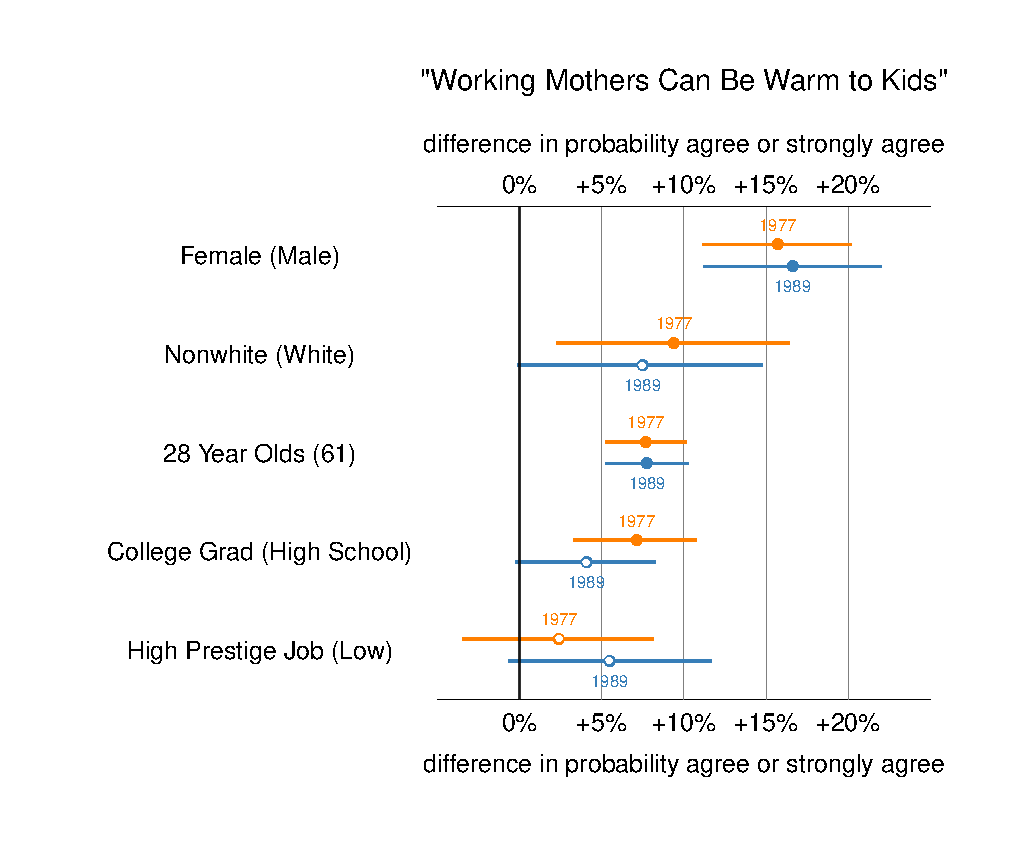
\includegraphics[width=0.7\textwidth]{plots/mothersFD7789.pdf} 
      \vspace{-2.5em}
      \caption{\textbf{This table is floating between texts} Solid lines represent the simulated change...}
      \label{fig:FloatingPlot}
  \end{center}
\end{figure} 



In 1995, as Figure~\ref{fig:FloatingPlot} suggests, Ichiro led the Blue Wave to its first Pacific League pennant in 12 years. In addition to his second batting title, he led the league with 80 RBI and 49 stolen bases, while his career-high 25 home runs were third in the league. By this time, the Japanese press had begun calling him the "Hit Manufacturing Machine". The following year, with Ichiro winning his third-straight MVP award, the team defeated the Central League champion, Yomiuri Giants, in the Japan Series. Following the 1996 season, playing in an exhibition series against a visiting team of Major League All-Stars kindled Ichiro's desire to travel to the United States to play in the Major Leagues.

In November 1998, Ichiro participated in a seven-game exhibition series between Japanese and American all-stars. Ichiro batted .380 and collected seven stolen bases in the series, winning praise from several of his MLB counterparts, including Sammy Sosa and Jamie Moyer (who would become his teammate with the Mariners).

\begin{figure}[t] % But I like to place on top
  \begin{center}
      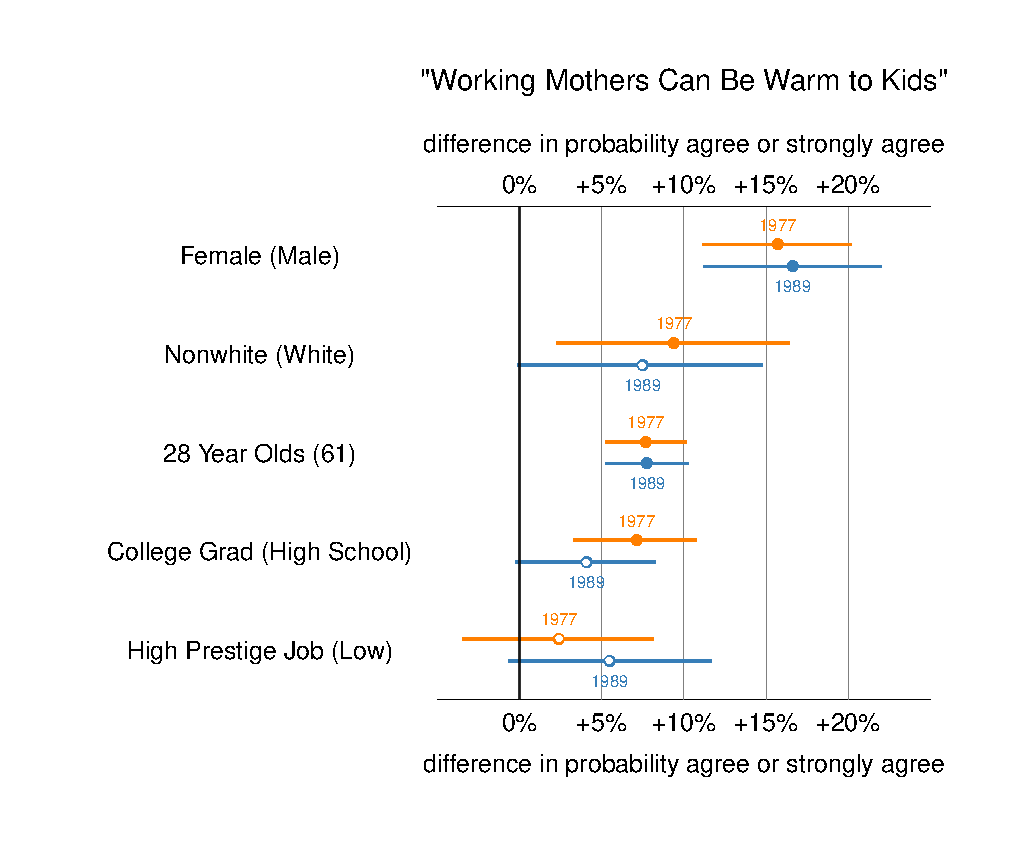
\includegraphics[width=0.7\textwidth]{plots/mothersFD7789.pdf} 
      \vspace{-2.5em}
      \caption{\textbf{This table is Located at Top.} Solid lines represent the simulated change...}
      \label{fig:TopPlot}
  \end{center}
\end{figure} 

In 2000, Ichiro was still a year away from being eligible for free agency, but the Blue Wave was no longer among Japan's best teams. Because the team would probably not be able to afford to keep him, and would lose him without compensation in another year, Orix allowed him to negotiate with Major League clubs. Ichiro used the posting system, and the Seattle Mariners won the right to negotiate with him with a bid of approximately $13 million.[12] In November, Ichiro signed a three-year, $14 million contract with the Seattle Mariners. In his nine NPB seasons in Japan, Ichiro had 1,278 hits, a .353 career batting average, and won seven Golden Glove Awards. Ichiro's time in the Japanese baseball leagues matured him as a player and a person, and he often credits it for his success.

\section{Random Useful Resources}
Bib \\
\url{http://merkel.texture.rocks/Latex/natbib.php} \\
Gary King's bib\\
\url{https://github.com/iqss-research/gkbibtex/blob/master/gk.bib}\\
Math\\
\url{https://en.wikibooks.org/wiki/LaTeX/Mathematics}\\

\clearpage


%%%%%%%%%%%%%%%%%%%%
%%% Bibliography %%%
%%%%%%%%%%%%%%%%%%%%

\bibliography{references}

\clearpage

%%%%%%%%%%%%%%%%%%%%
%%%%% Appendix %%%%%
%%%%%%%%%%%%%%%%%%%%


\appendix
\section*{Appendix}
\setcounter{secnumdepth}{0}
\setcounter{table}{0}
\setcounter{figure}{0}
\renewcommand{\thetable}{A\arabic{table}}
\renewcommand{\thefigure}{A\arabic{figure}}

\begin{figure}[tbh]
  \begin{center}
      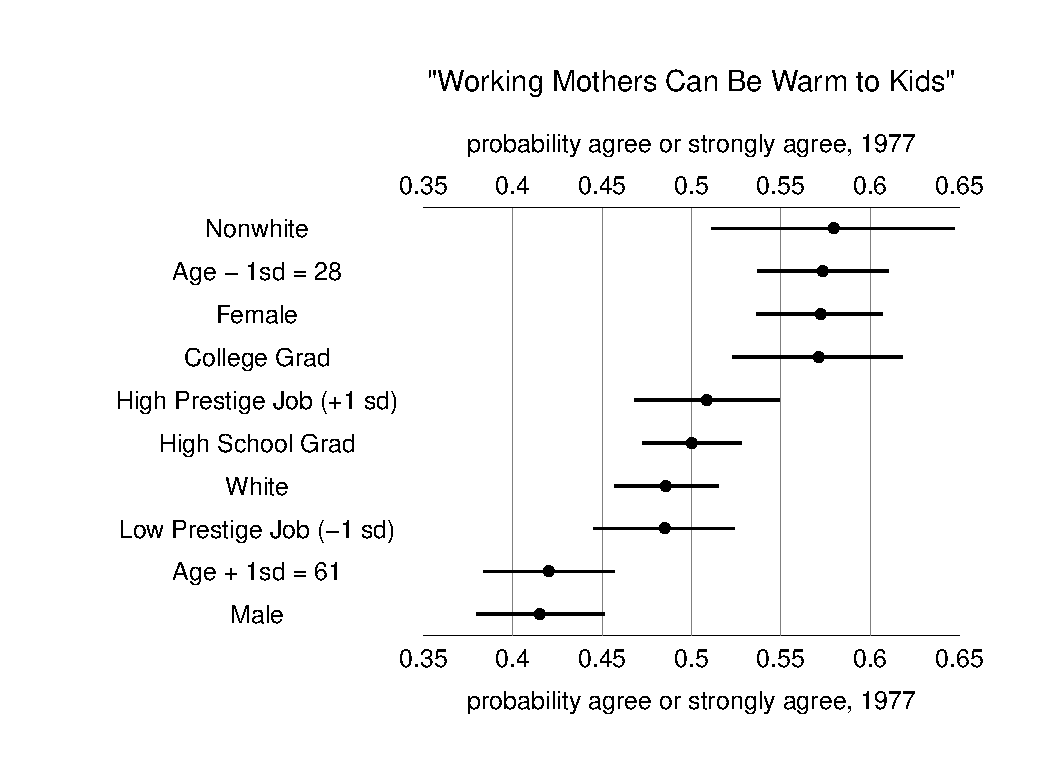
\includegraphics[width=1.05\textwidth]{plots/mothers1catEV.pdf}
      \vspace{-2.5em}
      \caption{\textbf{Expected Values for Models of Ordered Data.} Solid lines represent the simulated change in the liberal democracy index in year $t$, given a particular type of crisis happened once in year $t-i$, where $i \in \{1, 2, 3, 4, 5\}$, against some level of liberal democracy index in that year. Shaded regions represent 90\% confidence intervals, whereas dashed lines represent 95\% confidence intervals. All other control variables are lagged by 1 year (a lagged liberal democracy index by 1 year is also present in models where $i \neq 1$); country- and year-fixed effects are included in all models.}
      \label{fig:crises*libdem*time}
  \end{center}
\end{figure} 


\begin{landscape}
%\subsection{Appendix Tables and Figures}
\subimport{tables/}{tableA1.tex}
\end{landscape}






\end{document}